\documentclass[11pt,a4paper]{article}
\usepackage[margin=2.2cm]{geometry}
\usepackage{amsmath,amssymb}
\usepackage{graphicx}
\usepackage{booktabs,array}
\usepackage{float}
\usepackage[font=small,labelfont=bf]{caption}
\usepackage{xcolor}
\usepackage{listings}
\usepackage{adjustbox}
\usepackage[colorlinks=true,linkcolor=blue!50!black,urlcolor=blue!50!black]{hyperref}
\lstset{basicstyle=\ttfamily\small,columns=fullflexible,frame=single,backgroundcolor=\color{gray!8},breaklines=true}
\newcommand{\el}{\ensuremath{e^-}}
\newcommand{\AGMX}{A\_GMX}
\newcommand{\code}[1]{\texttt{#1}}
\setlength{\parskip}{4pt}
\setlength{\emergencystretch}{3em}
\graphicspath{{figures_crowded/}}

\title{\textbf{\AGMX{} on crowded CCDs}\\[4pt]
\large background override, serial-register streaks, straight-track hints, crossing split and track linking}
\author{comm\_scripts clustering study}
\date{code of 29 October 2026 (\code{clustering\_tests/crowded.py})}

\begin{document}
\maketitle

\begin{abstract}
On CCDs where tracks cover a large part of the image (surface runs such as L2 ACM101, the Am-241 test CCD), \AGMX{} had
three failures: its row-by-row background fit picked the wrong whole-electron pedestal in rows with
$\sim$10\,\el/pix of dark charge; serial-register streaks were merged into tracks; and long straight tracks
(muons) were cut into several clusters wherever they crossed other tracks, while touching tracks were merged into star-shaped
clusters of up to $10^4$\,px. \emph{Crowded mode} fixes these and is switched on per image when the image is crowded. The
straight tracks are found by a separate finder, but only their \emph{axis} is passed to \AGMX{} as a hint: the cluster's
width, footprint and the charge shared with crossing tracks remain \AGMX's own. On L2, injected muons go from 4.1 fragments
and 45\,\% of their charge in one cluster to 1.9 fragments and 93\,\%; Fe-55 K$\alpha$ narrows from 220 to 85\,eV on the
worst CCD and gains 14--65\,\% events. On the Am-241 crowded CCD (EXT4) the energy scale of the constrained 10--30\,keV fit is
unchanged ($k=1.0004$ vs $1.0009$ on the same images), and on EXT3 too ($k=0.9952\pm0.0008$ vs $0.9964\pm0.0010$, 29 images)
once the fit is started from narrow line widths (section~\ref{sec:ext3}). Crowded mode is the default
(\code{crowded='auto'}): it runs only on images that pass the trigger, and other images are clustered as before.
\end{abstract}

\tableofcontents

%======================================================================================================
\section{When is an image crowded?}\label{sec:trigger}
The trigger is the \emph{core fill}: the fraction of active pixels whose charge, smoothed with a Gaussian of 1\,px, exceeds
$\max(60\,\el,\,5\,\sigma_\lambda)$, where $\sigma_\lambda=\sqrt{\lambda}/(2\sqrt\pi)$ is the noise of the smoothed dark
charge $\lambda$. It measures how much of the CCD is covered by deposits, independent of the background level.
\begin{center}\small
\begin{tabular}{lcc}
\toprule
image type & core fill & crowded mode with \code{auto} \\ \midrule
L2 ACM101 surface run (EXT1/2/4) & 0.27--0.31 & on \\
Am-241 AMTest EXT3 / EXT4 & 0.27 / 0.43--0.67 & on \\
Fe-55 production CCDs (gn\_lowcharge\_study) & 0.015--0.02 & off \\
\bottomrule
\end{tabular}
\end{center}
\code{crowded='auto'} switches crowded mode on for core fill $\ge0.10$; \code{'on'} and \code{'off'} force it. Below the
threshold nothing in this note runs, and \AGMX{} output is identical to the code without crowded mode (unit test).

%======================================================================================================
\section{The five pieces}

\subsection{Background override (only at high dark charge)}
\AGMX's background model fits each row with a Poisson$\otimes$Gaussian (offset $o$, dark charge $\lambda$, noise $s$). With
$\lambda\gtrsim5$\,\el/pix the zero-electron peak is gone and $o$ is only known modulo whole electrons: on L2 EXT1, 395 of 500
rows took a pedestal 4--85\,\el{} too high, which made energies wrong by up to $-6$\,\el/pix $\times$ the cluster area and
produced a 10--160k\,px ``blob''. The override:
\begin{enumerate}
\item is applied only for electron-counting images (median $s<0.45$\,\el) with median $\lambda\ge3$\,\el/pix;
\item flags a row as bad when more than 0.5\,\% of its pixels lie below $o-0.5-3s$, and gives it the whole-electron
pedestal of the good rows (keeping its fractional part);
\item re-estimates $\lambda$ in cells of $10\times64$\,px by a truncated-Poisson fit below the 90\,\% quantile (so that the
halos of tracks do not raise it), and overrides the row model where the two differ by more than
$\max(0.3,\,5\sigma)$\,\el/pix; bad rows take the cell value.
\end{enumerate}
The gate on $\lambda$ matters: on Am-241 ($\lambda=0.2$--2.4\,\el/pix) the dense X-ray field fools both tests (EXT3: 40--70\,\%
of the cells changed, energies $-0.2$\,\%, 59.5-keV events lost; EXT4: 429 ``bad'' rows and backgrounds of $10^4$\,\el/pix).
A unit test checks that the override never moves a row's pedestal away from the truth.

\paragraph{Hot-column bands.} On L2 9 EXT1 columns 893--925 carry $+8$\,\el/pix of extra dark charge with sharp edges;
the 64-column cells cannot follow them and \AGMX{} turned the band into 700--3000\,px faint ``blobs''. For every column and
block of 32 rows the mean of the free pixels (deposits above $8\sigma$ masked) minus the model is measured, smoothed along
the column only, and added to $\lambda$ where it is positive, $\ge\max(2\,\el,\,4\sigma)$ and part of a run of $\ge4$ adjacent
columns. Coherent \emph{deficits} are not applied: they sit in rows with undershoot after bright tracks, where the
low-count statistics still fit the row model. Fe-55 on L2 is unchanged (EXT1 gains 3\,\% events).
\paragraph{Glow flag.} Clusters of $\ge100$\,px whose mean charge per pixel is below $3\sqrt\lambda$ are background structure
the model does not follow: class \code{glow} (\code{agmx\_cls} = 11), 5--12 per L2 CCD.

\subsection{Serial-register streaks}
Charge clocked into the serial register lands in one row with no vertical spread. A significant pixel is \emph{single-row}
when the pixels above and below hold $<25$\,\% of its charge; horizontal runs of $\ge8$ such pixels (1-px gaps bridged; pieces
$\le10$\,px apart in a row joined) are removed from the image before clustering and reported as clusters with class
\code{artifact-row} and regime \code{serial} (\code{agmx\_regime} = 3).

\subsection{Straight-track hints}
\paragraph{Finding.} The \emph{core} (as in section~\ref{sec:trigger}) is reduced to its 1-px skeleton; a Hough transform in
tiles of $160\times160$\,px (half overlapping; votes summed over 3 neighbouring $\rho$ bins so that a wobbling skeleton still
counts) gives candidate lines with $\ge40$ votes. Lines within $10^\circ$ of a row are left to the streak finder. Each
candidate is refined (charge-weighted PCA of the core pixels within 2\,px) and walked along the image in both directions. A step
is occupied when a core pixel within $\pm1$\,px of the axis is a transverse ridge (its smoothed charge at least twice the
smaller of the two values at $\pm3.5$\,px) or lies on a track already accepted (so crossings do not stop the walk); the walk ends
after 6 empty steps.
\paragraph{Accepting.} A line is a straight track if it is $\ge40$\,px long, $\ge85$\,\% occupied, its median transverse rms is
$\le2.2$\,px, it is not a duplicate, and its charge is \emph{continuous}: of the steps along the axis, at most 15\,\% may lie
below half and at most 8\,\% below 0.3 of the median axis charge. The continuity test separates muons (injected: 90th percentile
0.09) from chains of X-ray blobs in a dense field (Am-241: 10th percentile 0.17); without it the finder took 166 ``tracks'' on an
Am-241 image, with it 13 (figure~\ref{fig:amtubes}).
\paragraph{Using the hints.} Nothing is removed from the image. \AGMX{} runs as always (seeds, EM of the Gaussian clouds, merge
graph, island arbitration). Then, for each hint (axis centre $\mathbf c$, direction $\mathbf u$, extent $t_0..t_1$,
rms width $w$), every cloud $k$ with
\[ |(\boldsymbol\mu_k-\mathbf c)\cdot\mathbf n|\le\max(1.5,\,w),\qquad t_0-3\le(\boldsymbol\mu_k-\mathbf c)\cdot\mathbf u\le t_1+3 \]
($\mathbf n\perp\mathbf u$) goes into one cluster, unless it is elongated (axis ratio $\ge1.6$) at more than $30^\circ$ to the
hint, which makes it part of a crossing track. The cluster gets class \code{muon} and \code{straight\_track = True}. Because the
pixels' charge is still split by the mixture's responsibilities, a crossing track keeps its charge and stays one cluster, and the
muon's width is the width \AGMX{} fits (figure~\ref{fig:width}).

An earlier version cut a tube around each track out of the image and shared charge at crossings with an EM step of its own; its
tubes were twice as wide as the tracks (its width estimate collected neighbours and halos), it took X-rays lying on the muon's
path (5--8\,\% of the Fe-55 events on L2) and left crumbs. The hint version has none of these.

\subsection{Crossing split}
After the merge graph and after the island arbitration, a cluster whose clouds hold two straight lines (RANSAC on the cloud
centres, each $\ge20$\,px and $\ge3$ clouds) that cross as an X ($\ge20^\circ$, both continuing $\ge8$\,px past the crossing) is
split into the two tracks; clouds go to the nearer line.

\subsection{Track linking}
Collinear straight fragments of one track are joined (both pieces $\ge12$\,px, endpoints within $\max(2.5,\,1.5+0.01L)$\,px of
the longer piece's axis, parallel within $4^\circ$, gap $<15$\,px, or $<25$\,px for pieces $\ge30$\,px). Shorter pieces ---
photo-electron tracks of 59.5-keV gammas, X-rays --- are never joined (with 5\,px, Am-241 EXT3 lost 4\,\% of its 59.5-keV
events). Streaks are not linked.

%======================================================================================================
\section{Results}

\subsection{L2 surface run: maps}
\begin{figure}[H]\centering
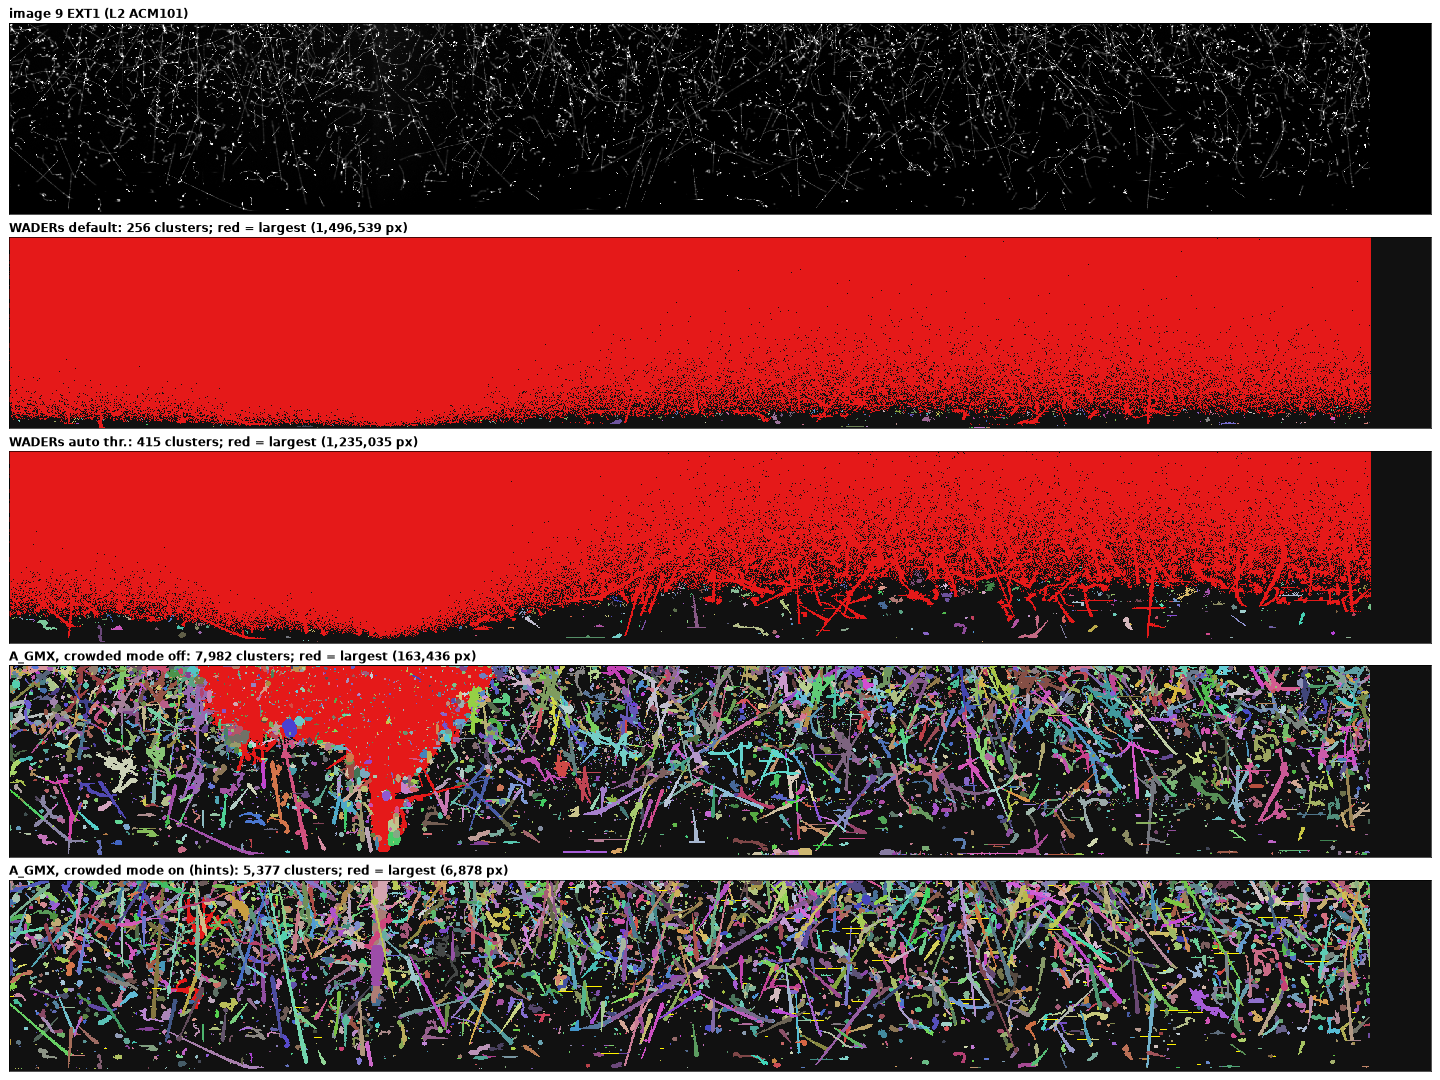
\includegraphics[width=\textwidth]{full_img9_ext1.png}
\caption{L2 image 9 EXT1. From the top: image; WADERs (default and electron thresholds: one cluster covers most of the CCD);
\AGMX{} without and with crowded mode. Red: the largest cluster; yellow: serial-register streaks.}
\end{figure}
\begin{figure}[H]\centering
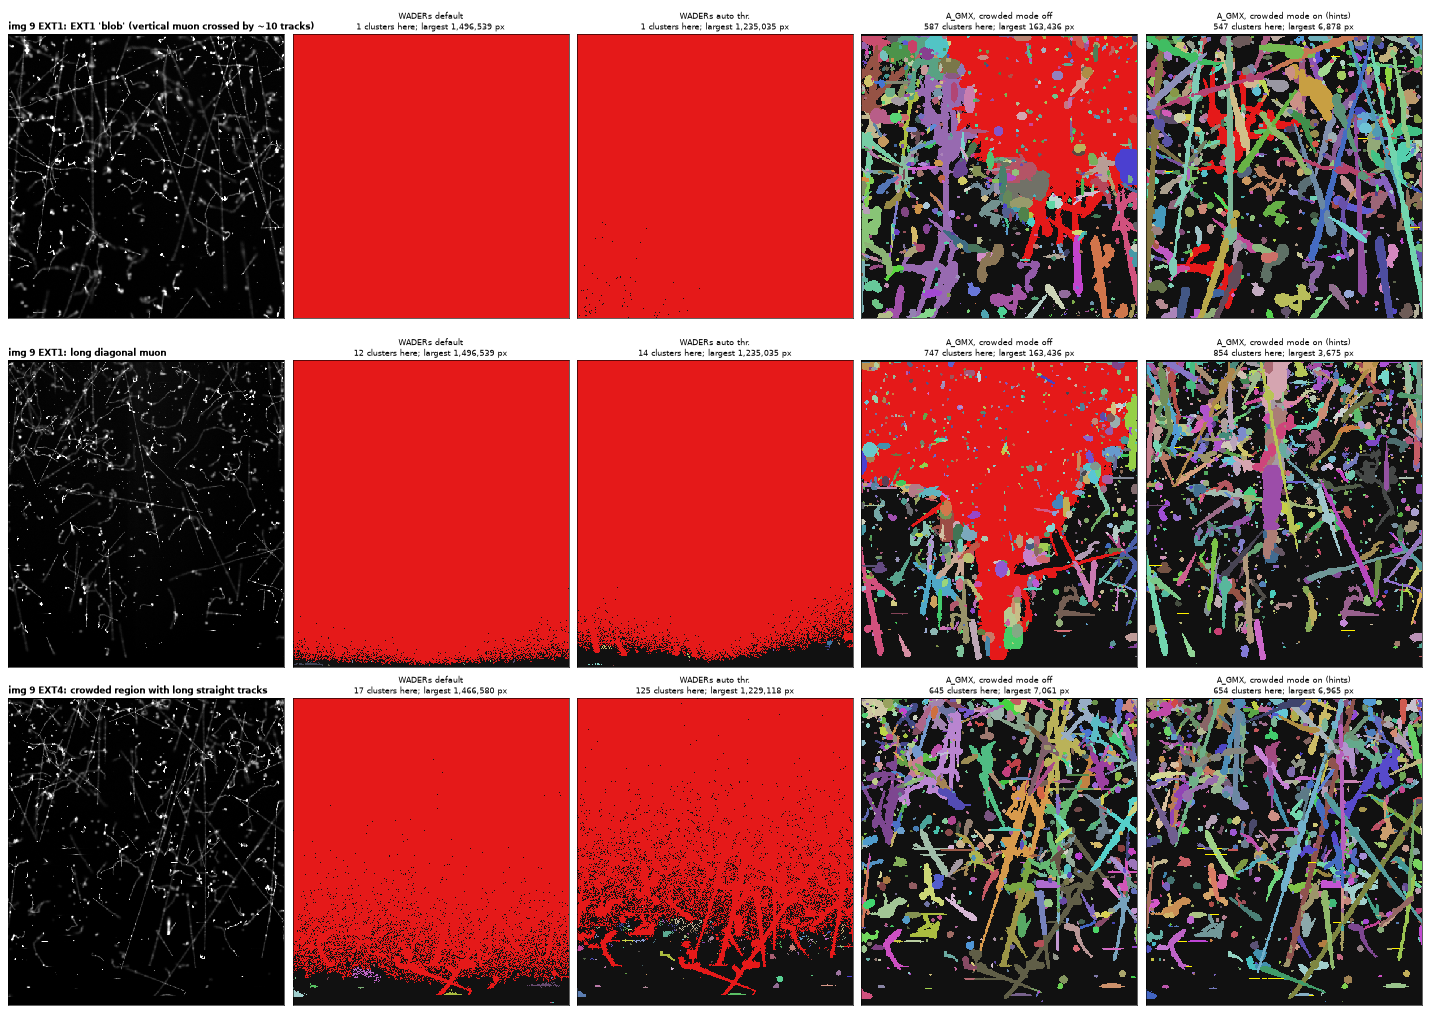
\includegraphics[width=\textwidth]{zoom_1.png}
\caption{Close-ups: the EXT1 ``blob'' (a vertical muon crossed by about ten tracks), a long diagonal muon, a crowded region of
EXT4. Columns as above; titles give the number of clusters in the cut-out and the largest.}
\end{figure}
\begin{figure}[H]\centering
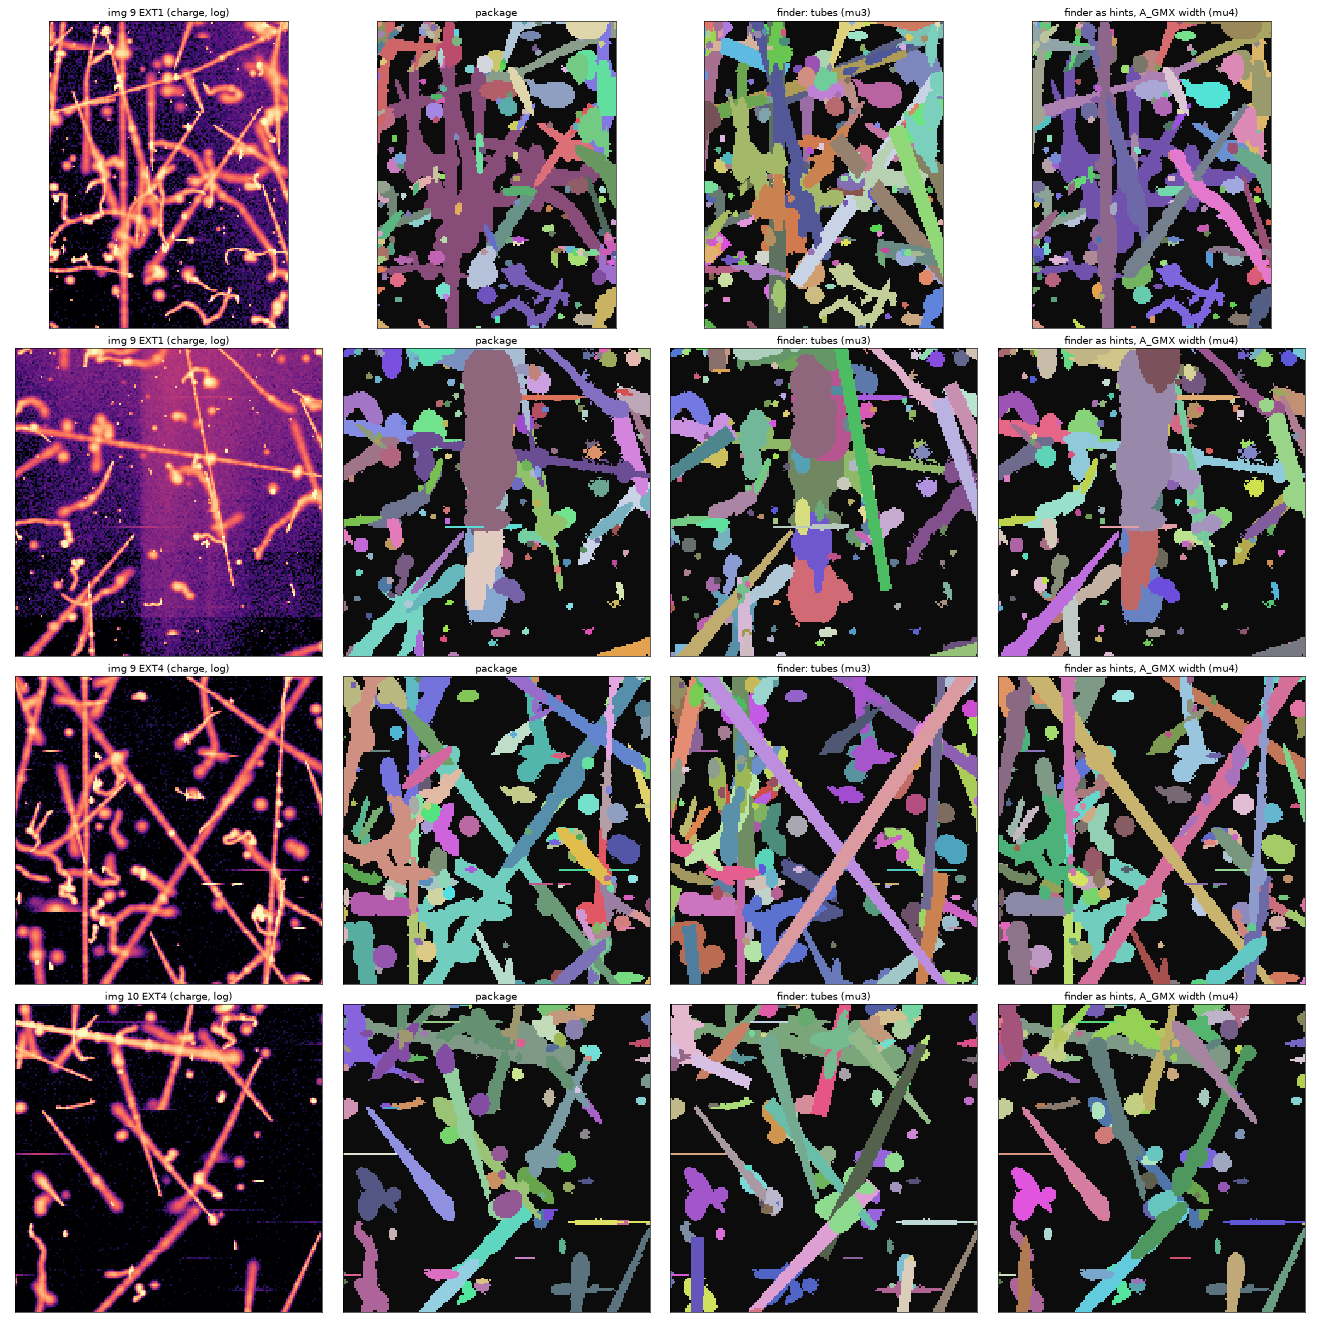
\includegraphics[width=0.95\textwidth]{width_zoom.png}
\caption{Track width. Columns: charge; the package without straight tracks; the earlier tube version (too wide); the hint
version, where the width is \AGMX's own.}\label{fig:width}
\end{figure}

\subsection{L2: injected muons}
25 muons per image (projected length 40--400\,px, Landau-fluctuating charge, diffusion growing from 0.2 to 0.8--1.6\,px
with depth) were added to the real L2 images 9 and 10 (EXT1, EXT4; 2 seeds: 200 muons) and the images clustered.
\begin{figure}[H]\centering
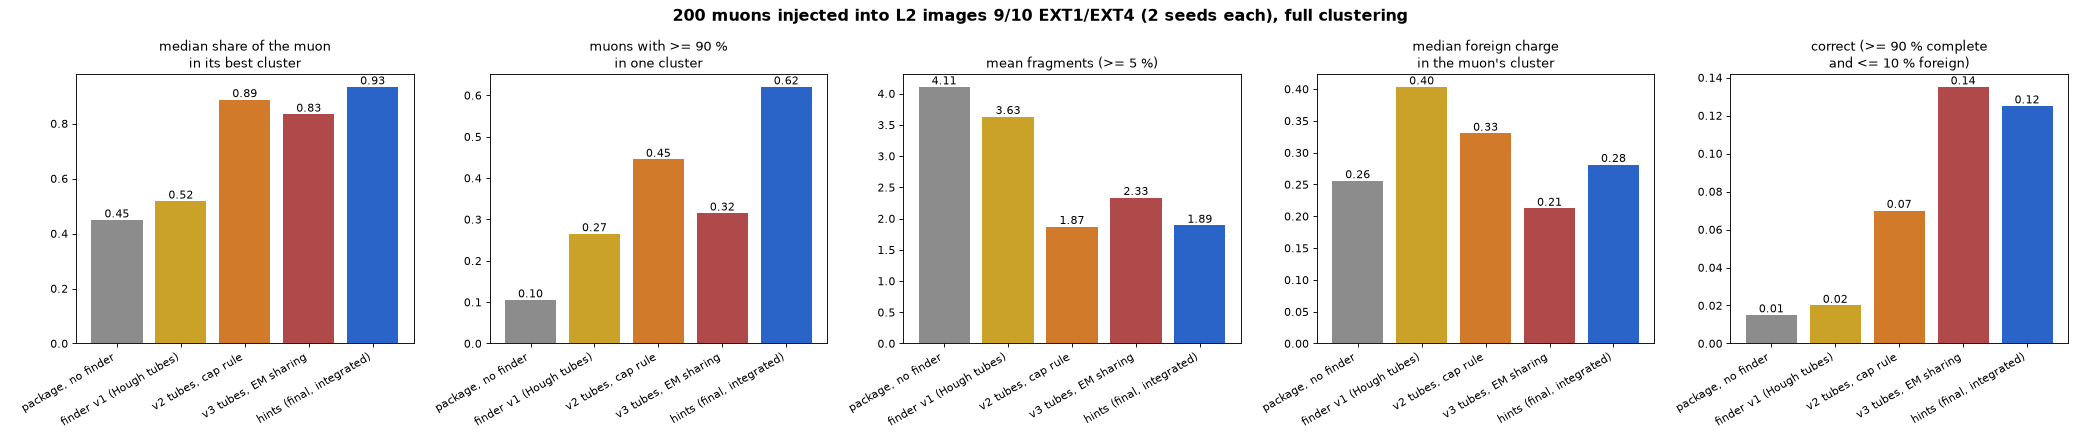
\includegraphics[width=\textwidth]{inj_bars.png}\\
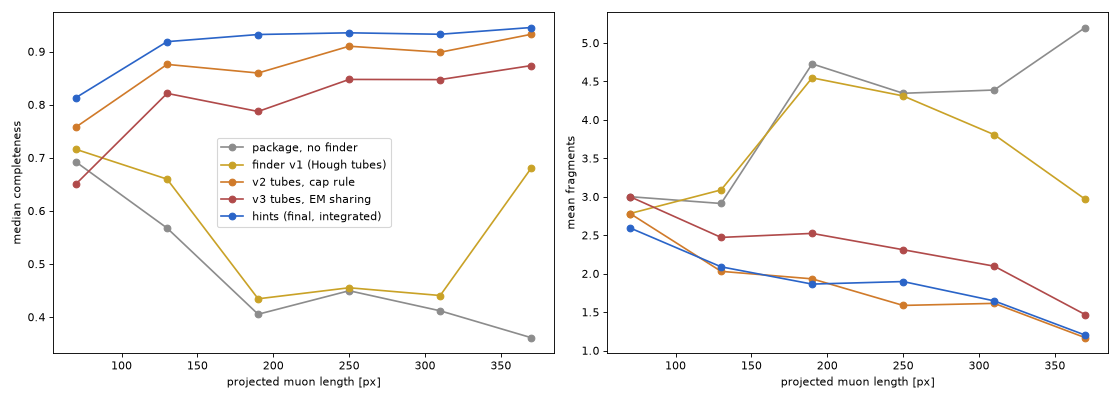
\includegraphics[width=0.6\textwidth]{inj_vs_length.png}
\caption{Per muon: share of its charge in its best cluster, fraction with $\ge90$\,\% in one cluster, number of fragments
($\ge5$\,\%), foreign charge in its cluster, and ``correct'' ($\ge90$\,\% in one cluster and $\le10$\,\% foreign). The last
bar is the final, integrated code. In this image a 300-px line crosses about 15 other tracks, so few muons can be ``correct''.}
\end{figure}
\begin{center}\small
\begin{tabular}{lccc}
\toprule
 & no straight tracks & tubes (earlier) & hints (final) \\ \midrule
median share in the best cluster & 0.45 & 0.83 & 0.93 \\
$\ge90$\,\% in one cluster & 10\,\% & 32\,\% & 62\,\% \\
fragments per muon & 4.1 & 2.3 & 1.9 \\
\bottomrule
\end{tabular}
\end{center}

\subsection{L2: Fe-55}
\begin{figure}[H]\centering
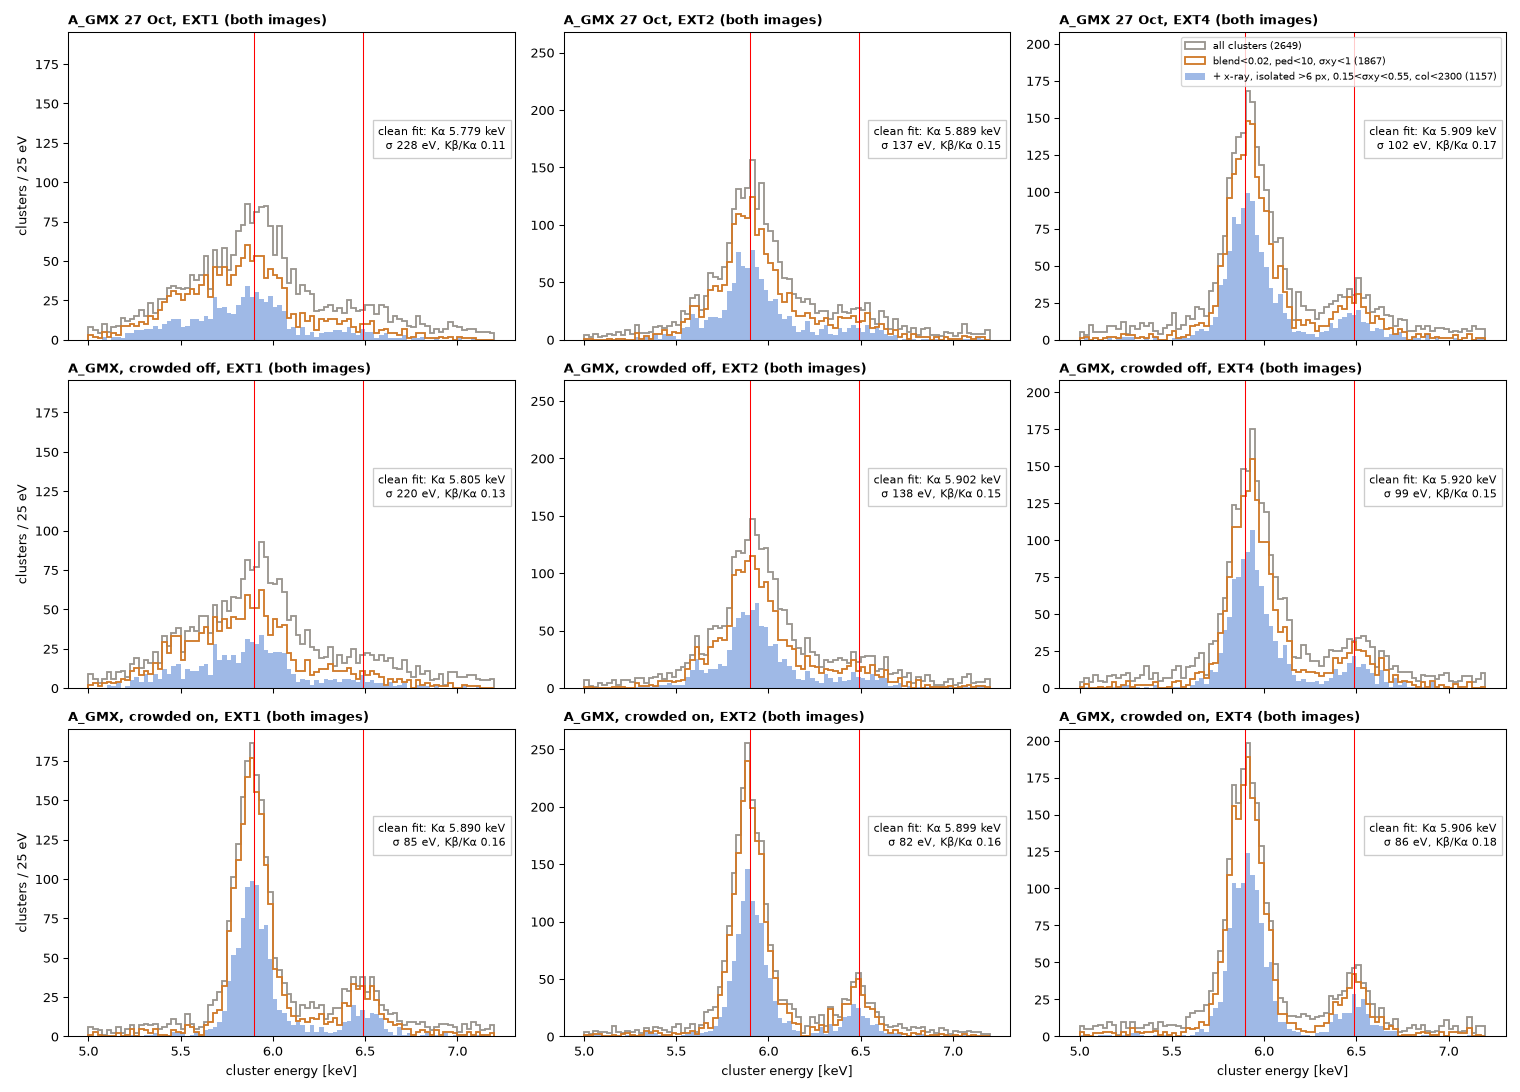
\includegraphics[width=\textwidth]{fe55_l2.png}
\caption{Fe-55 on L2 (images 9 and 10), front side. Rows: \AGMX{} of 27 October; today's \AGMX{} with crowded mode off;
with crowded mode on. Blue: clean selection (blend $<0.02$, ped $<10$, $\sigma_{xy}<1$, x-ray class, isolated $>6$\,px,
$0.15<\sigma_{xy}<0.55$, column $<2300$). Energies from 29 October use $\varepsilon(130\,\mathrm K)=3.7486$\,eV.}
\end{figure}
\begin{center}\small
\begin{tabular}{lccc}
\toprule
clean K$\alpha$ events / width & EXT1 & EXT2 & EXT4 \\ \midrule
crowded off & 476 / 220\,eV & 797 / 138\,eV & 896 / 99\,eV \\
crowded on & 785 / 85\,eV & 1016 / 82\,eV & 1021 / 86\,eV \\
\bottomrule
\end{tabular}
\end{center}

\subsection{Am-241, EXT4 (the crowded CCD)}
Ten of the 29 AMTest images (every third) were reclustered with crowded mode on and compared with the \AGMX{} clusters of
27 October on the same images (energies scaled to the same $\varepsilon$).
\begin{figure}[H]\centering
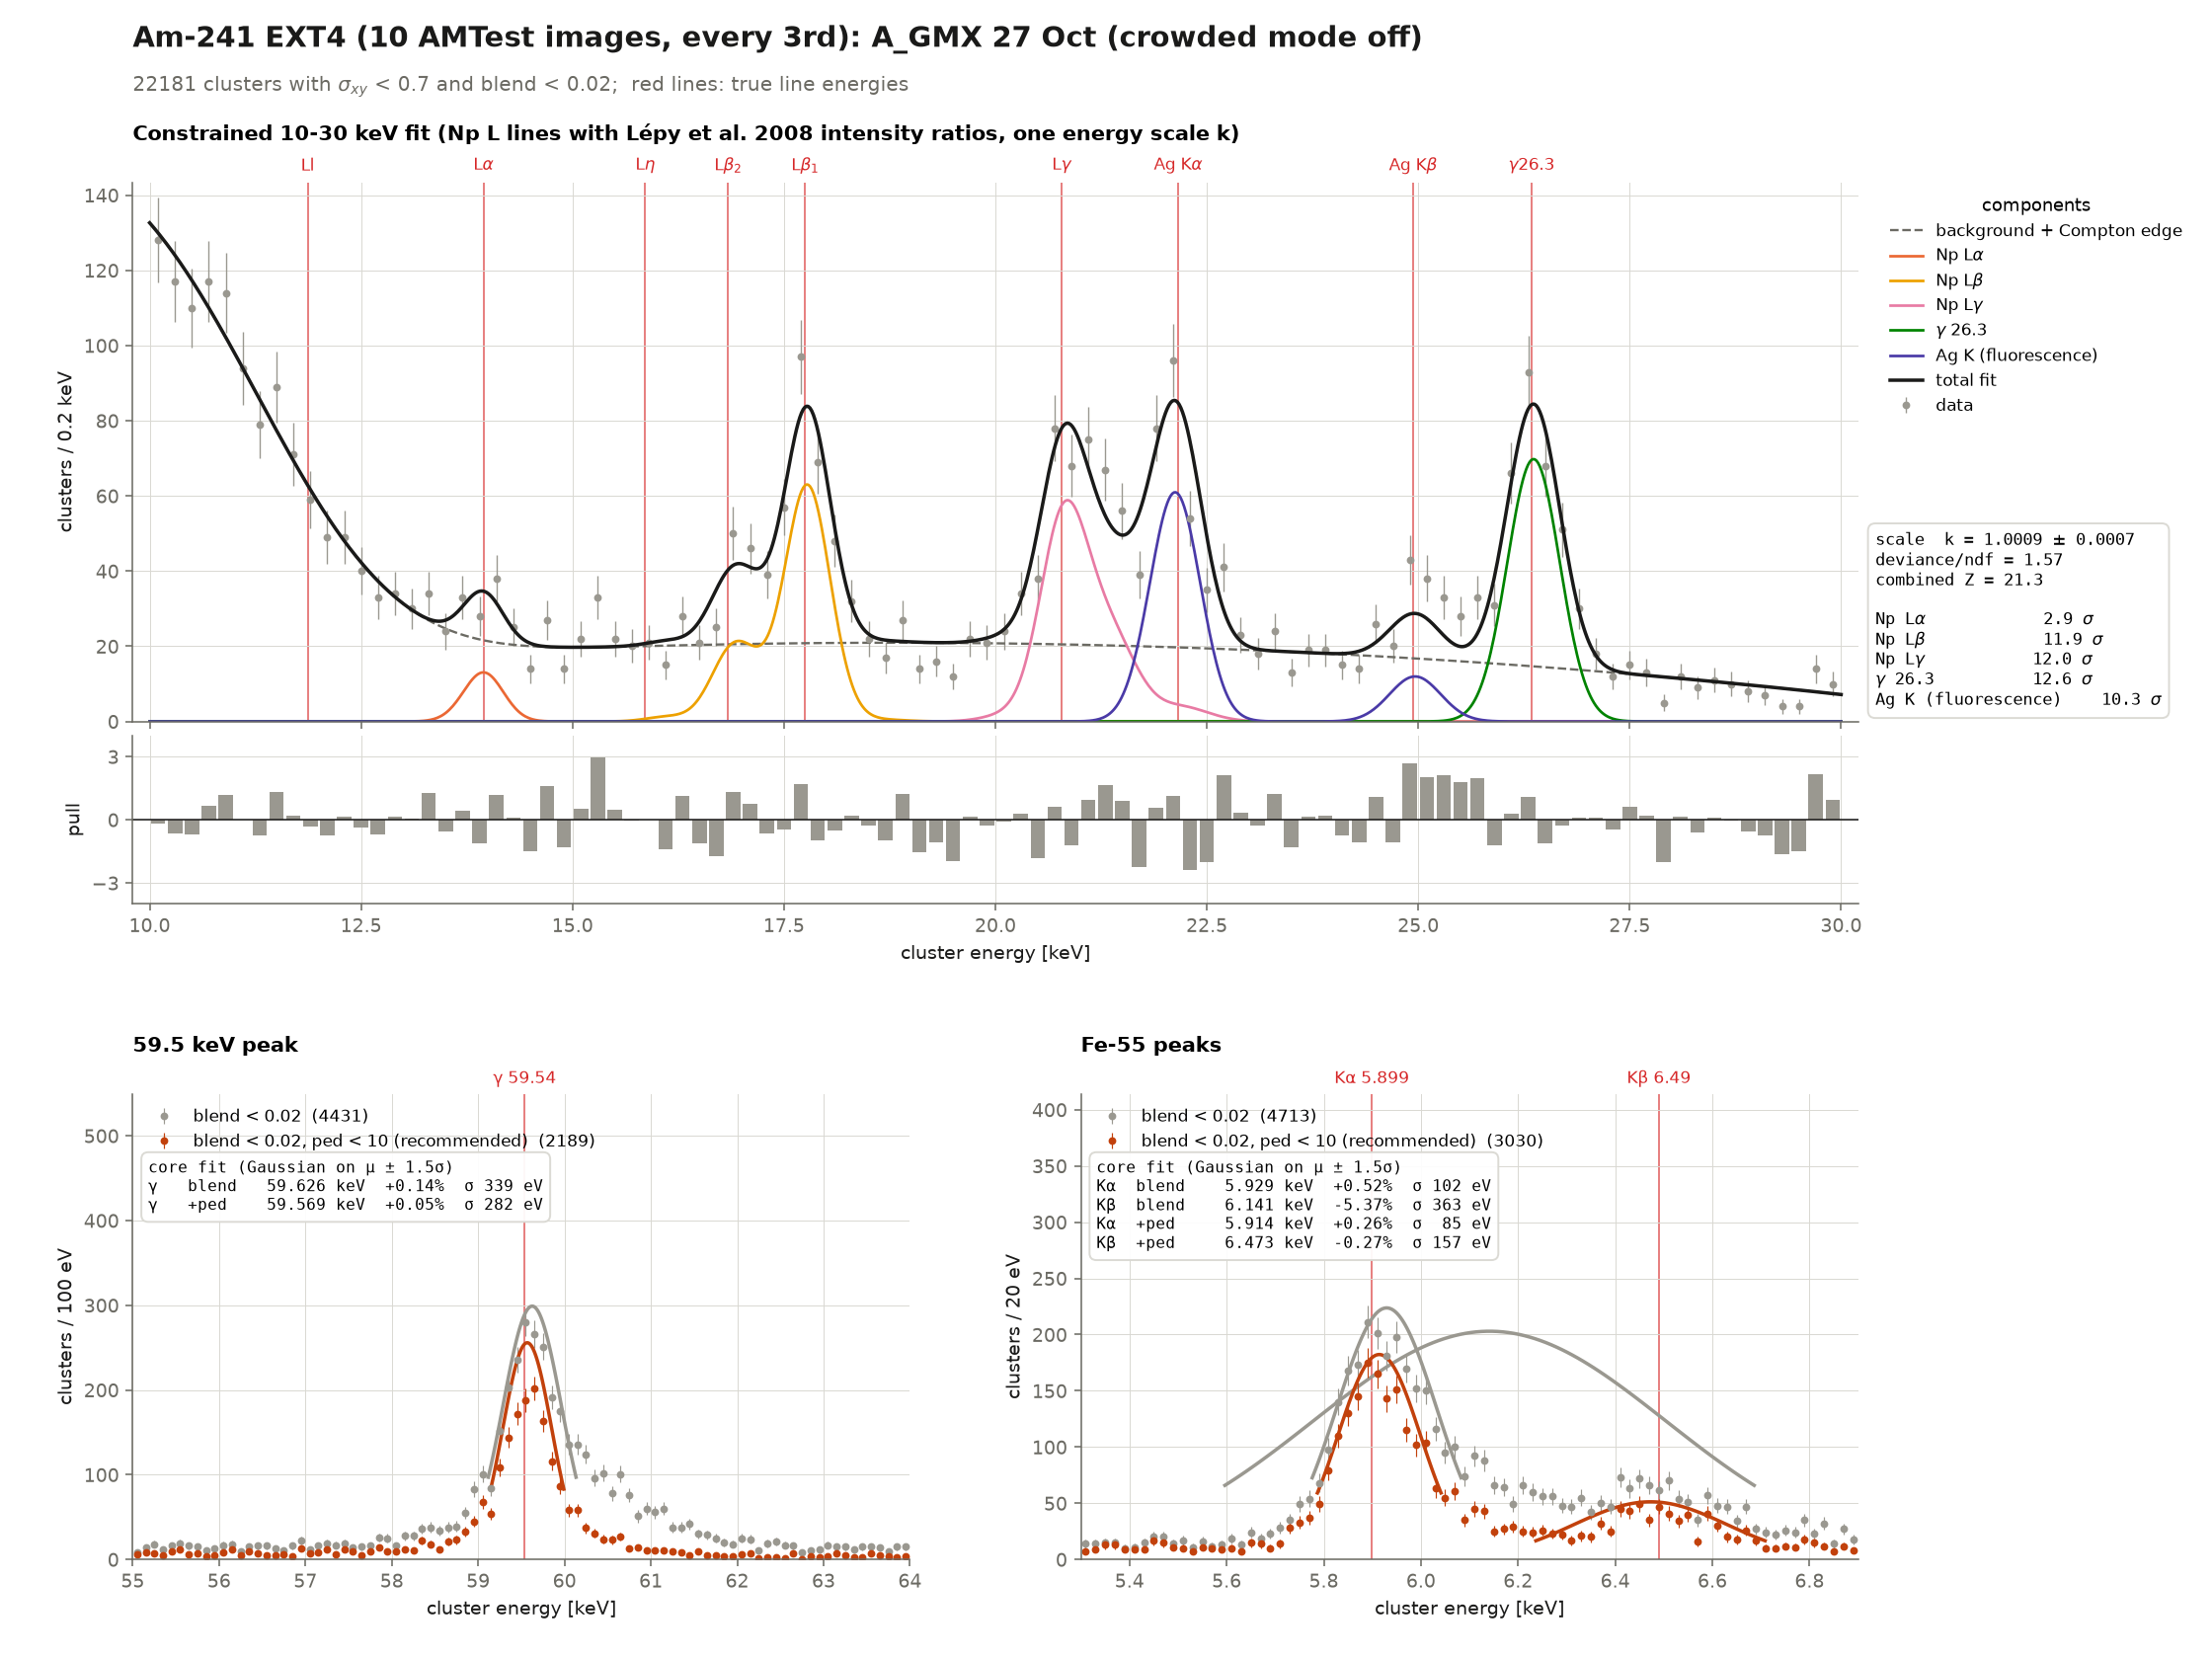
\includegraphics[width=0.49\textwidth]{fit_ext4_agmx27oct_sub10.png}\hfill
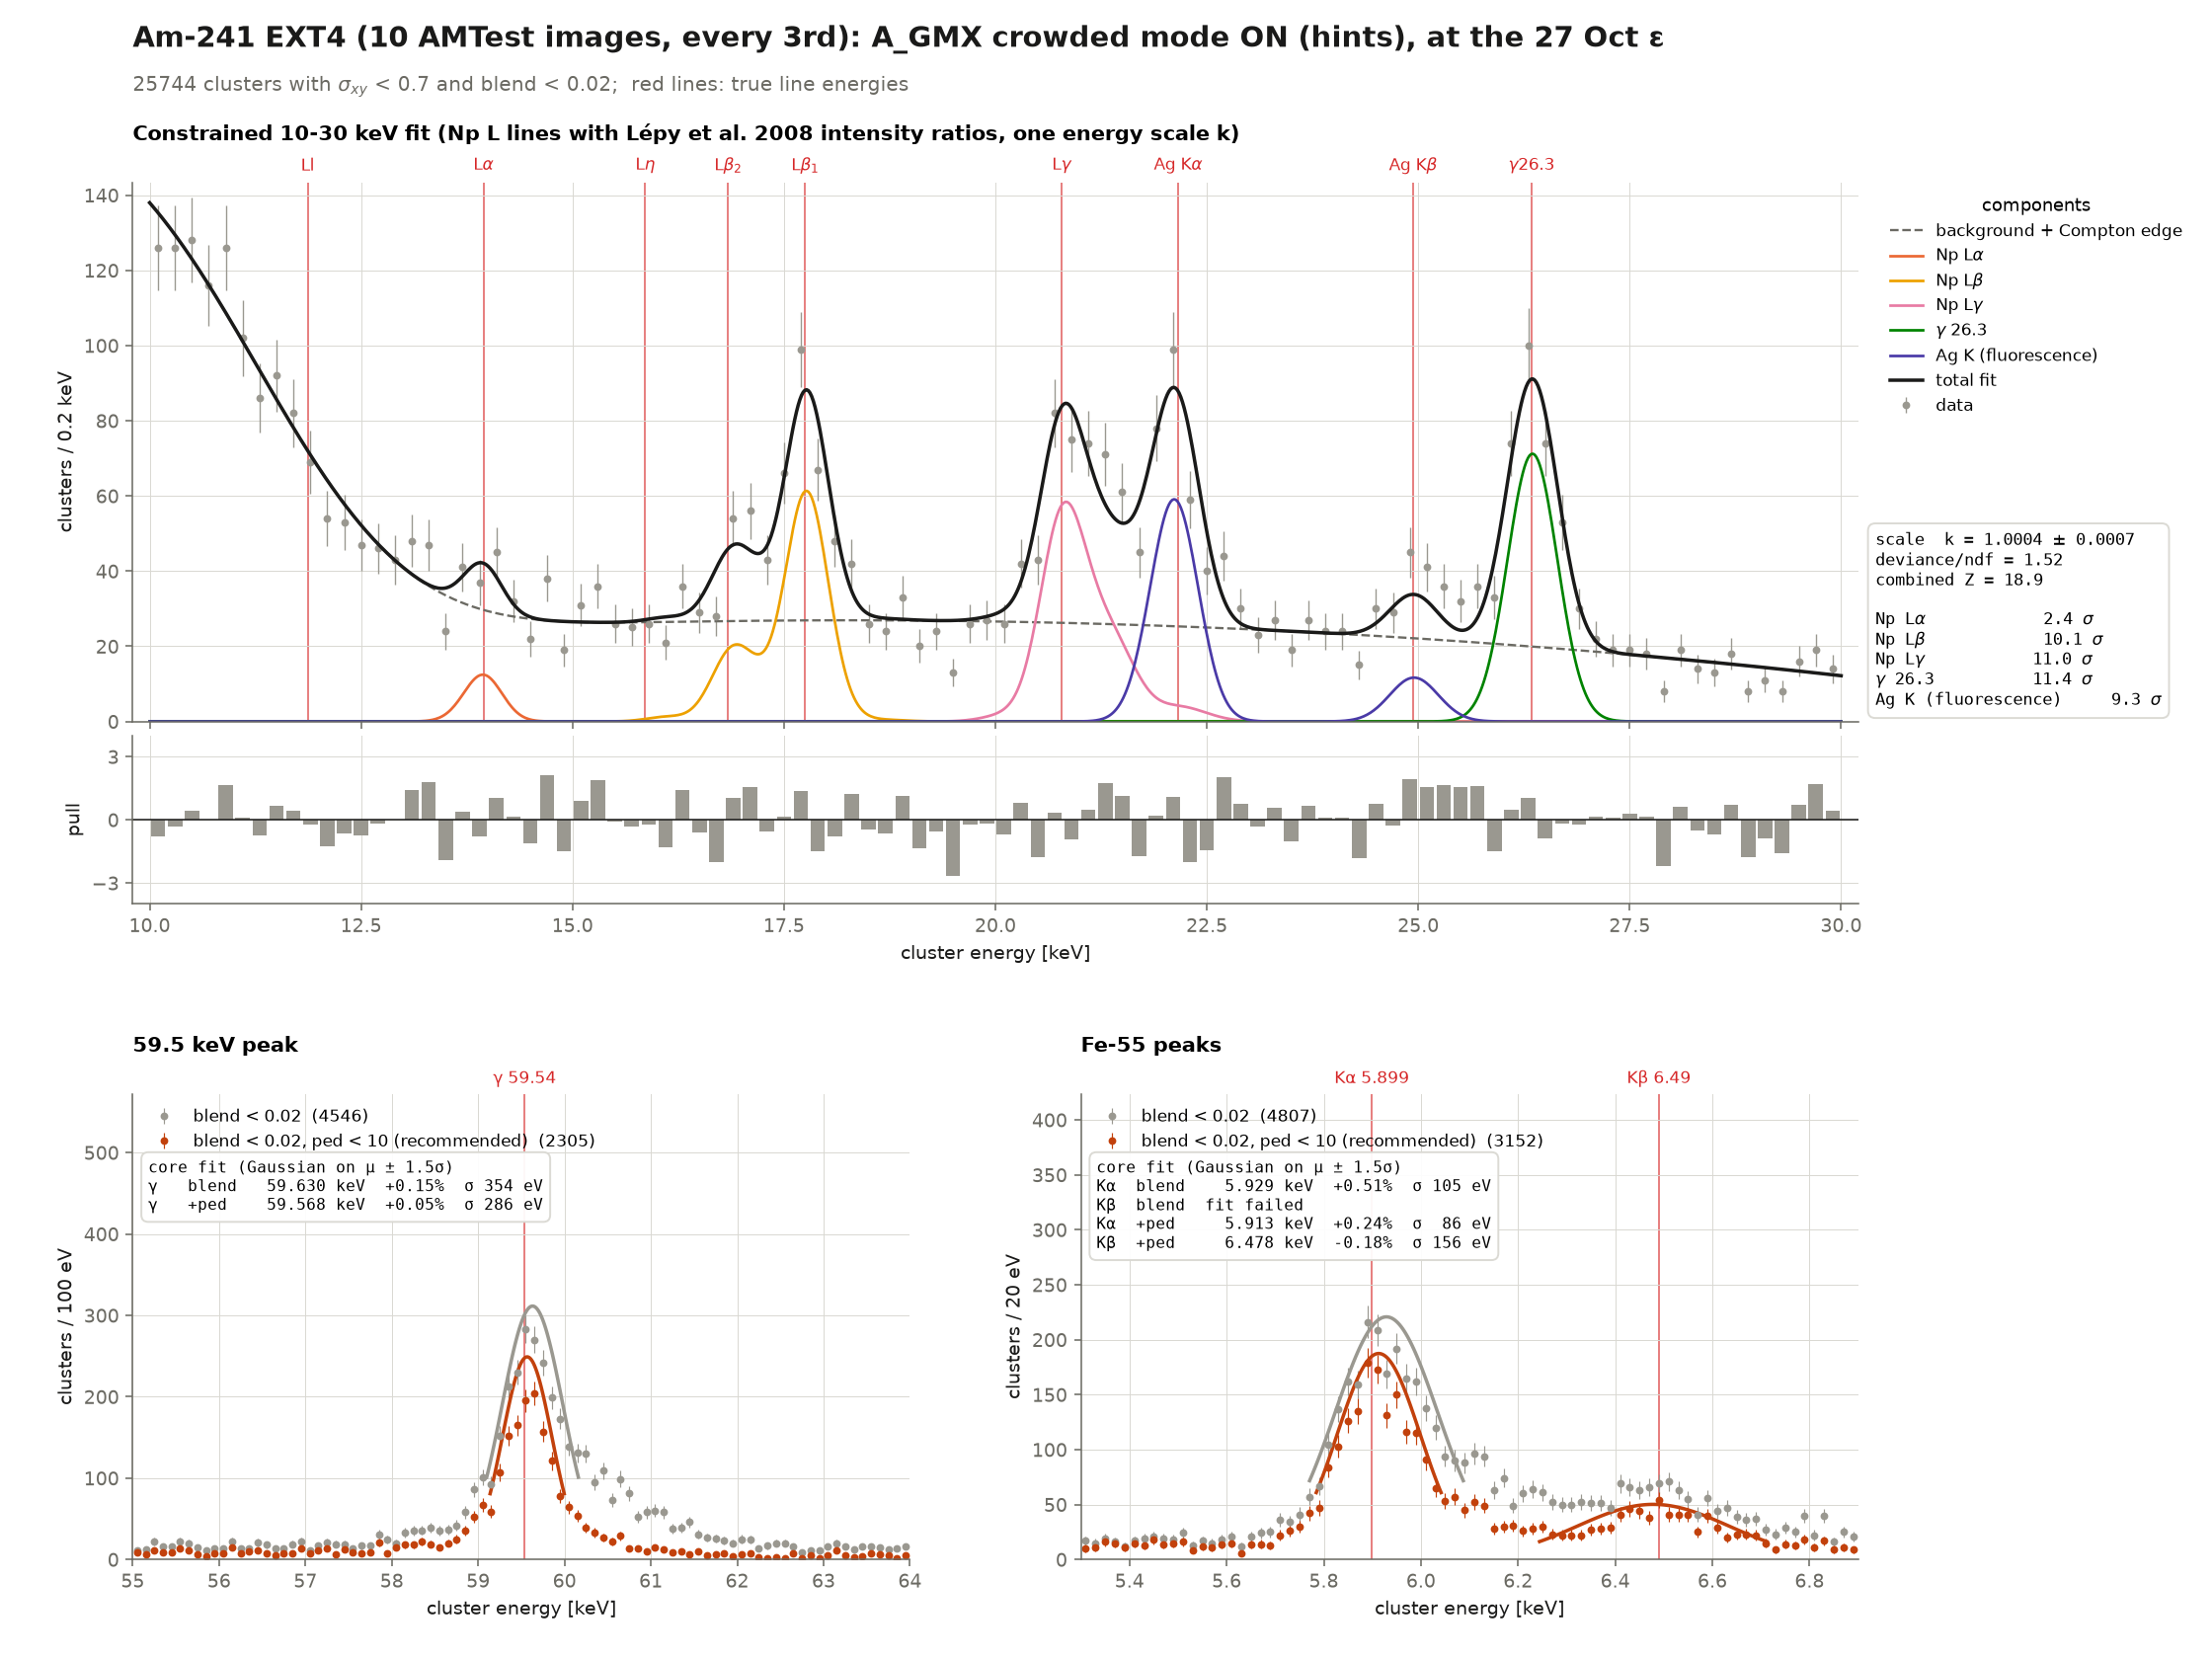
\includegraphics[width=0.49\textwidth]{fit_ext4_crowded_sub10.png}
\caption{Constrained 10--30\,keV fit (Np L lines with Lépy et al.\ intensity ratios, one energy scale $k$), 59.5-keV and
Fe-55 peaks. Left: without crowded mode ($k=1.0009\pm0.0007$, $Z=21.2$, 22\,181 clusters); right: with crowded mode
($k=1.0004\pm0.0007$, $Z=19.3$, 25\,744 clusters).}
\end{figure}
\begin{figure}[H]\centering
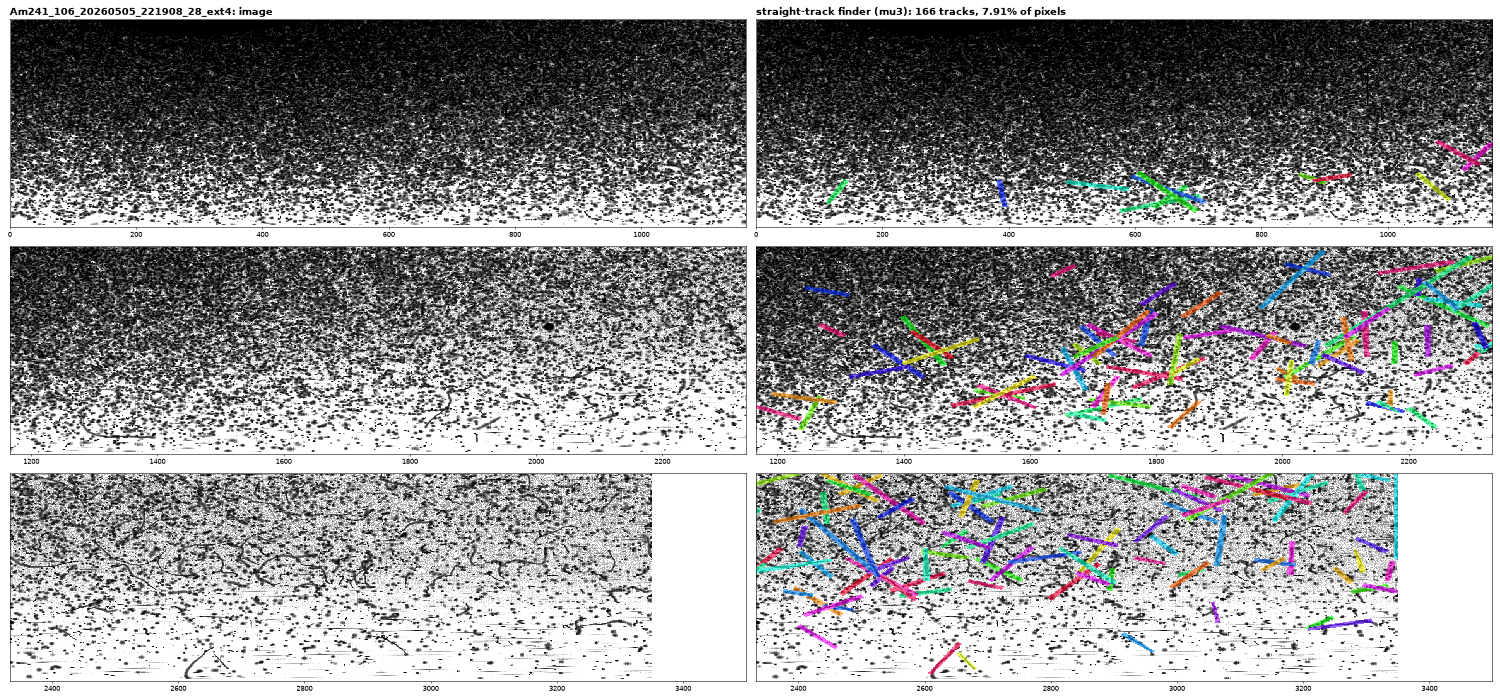
\includegraphics[width=0.49\textwidth]{tubes_am241_nocut.png}\hfill
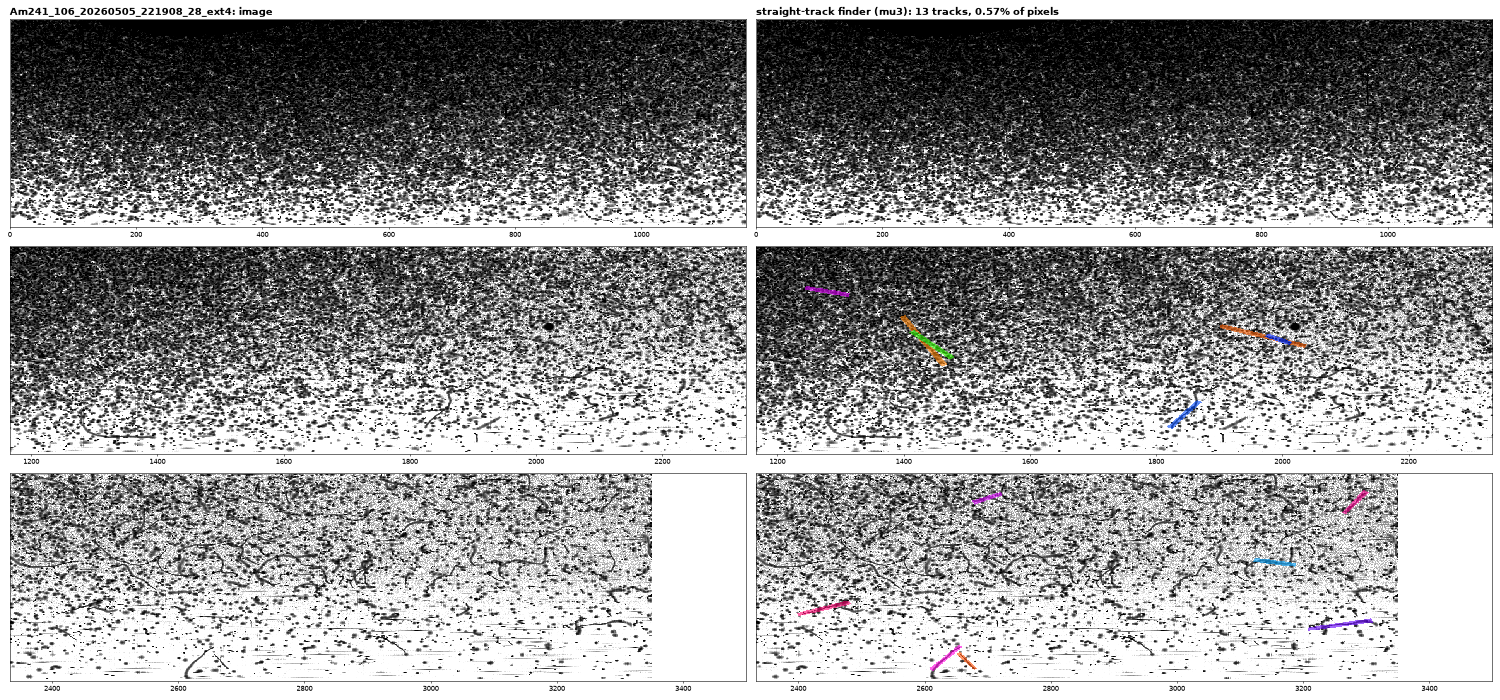
\includegraphics[width=0.49\textwidth]{tubes_am241.png}
\caption{Straight tracks on an Am-241 EXT4 image without (left, 166) and with (right, 13) the continuity test.}\label{fig:amtubes}
\end{figure}

\subsection{Am-241, EXT3}\label{sec:ext3}
With crowded mode the fit routine (\code{amfit.Model.fit}, 9 starts) first returned broad lines at the upper bound of the
width ($s_0=0.8$\,keV, $k=0.973$, $Z=4.7$). That was a local minimum: starting from narrow widths held fixed and then freed
gives a likelihood higher by $\Delta\ln L=42$ with $s_0=0.05$\,keV, the same as without crowded mode. The figures use this
extended start. Crowded mode adds 7--12\,\% events to the Np L lines and 26.3\,keV and removes 2.8\,\% at 59.5\,keV (with the
59.5-keV width 21\,eV narrower).
\begin{figure}[H]\centering
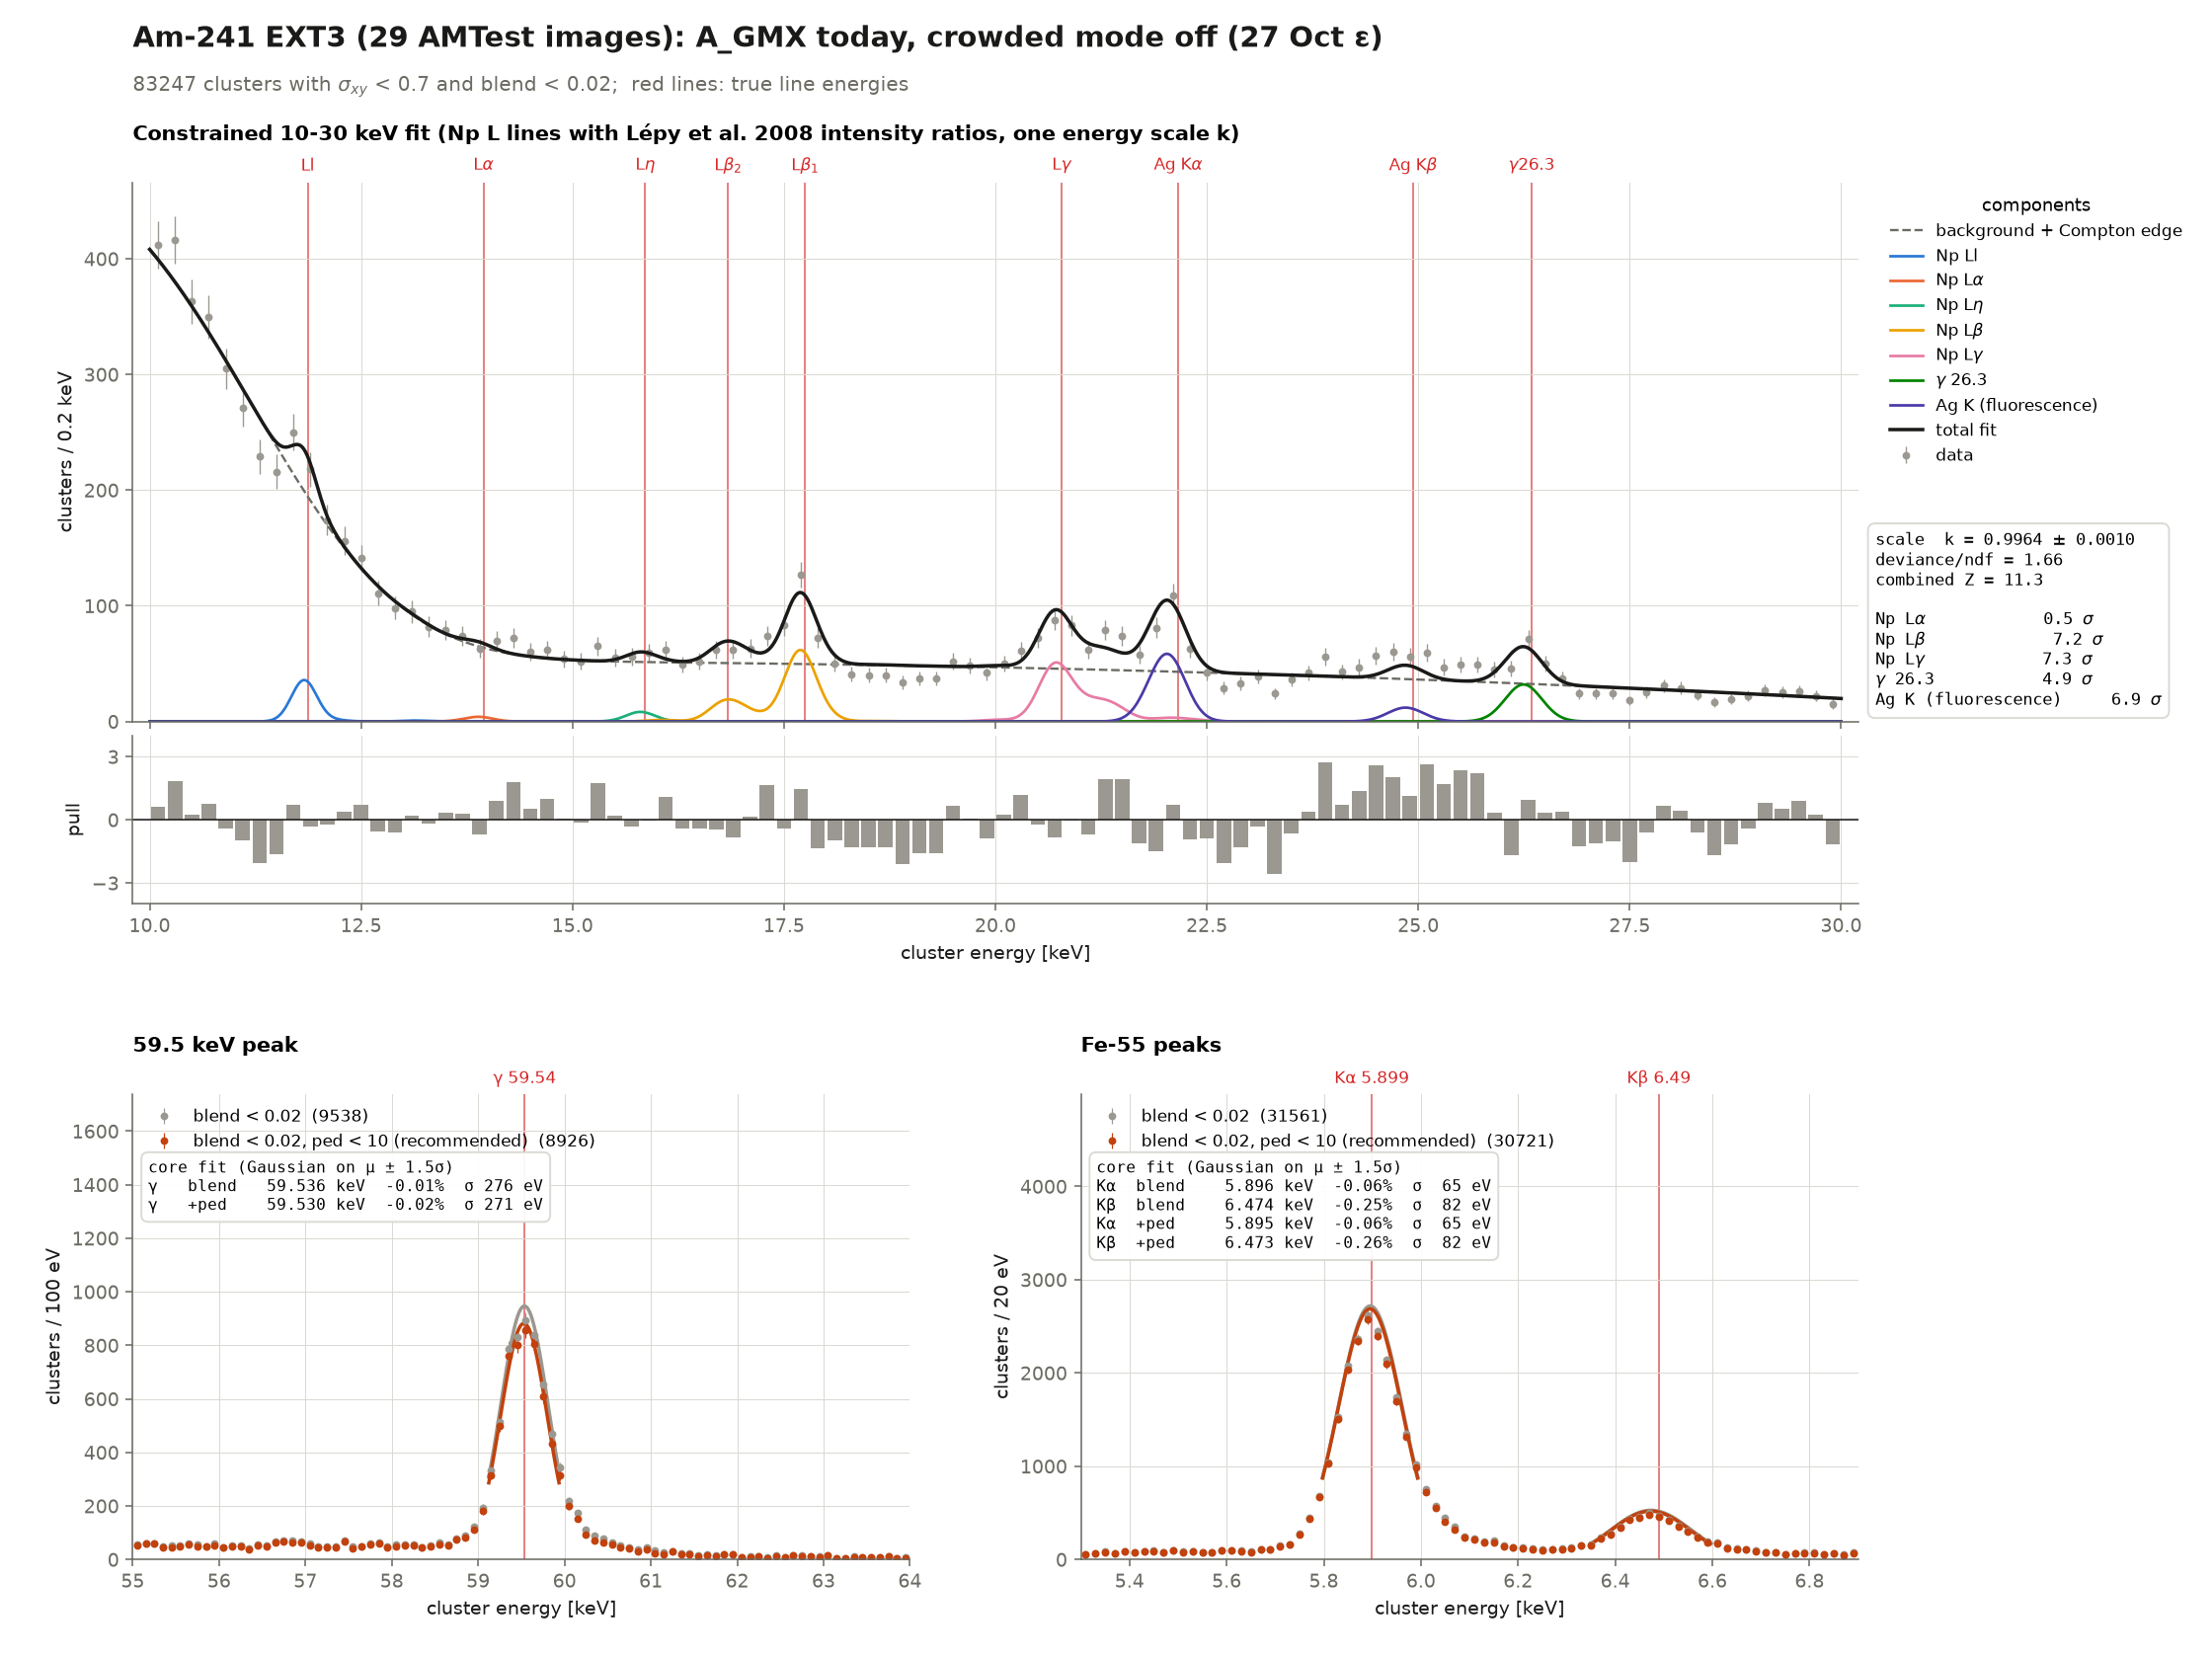
\includegraphics[width=0.49\textwidth]{fit_ext3_off.png}\hfill
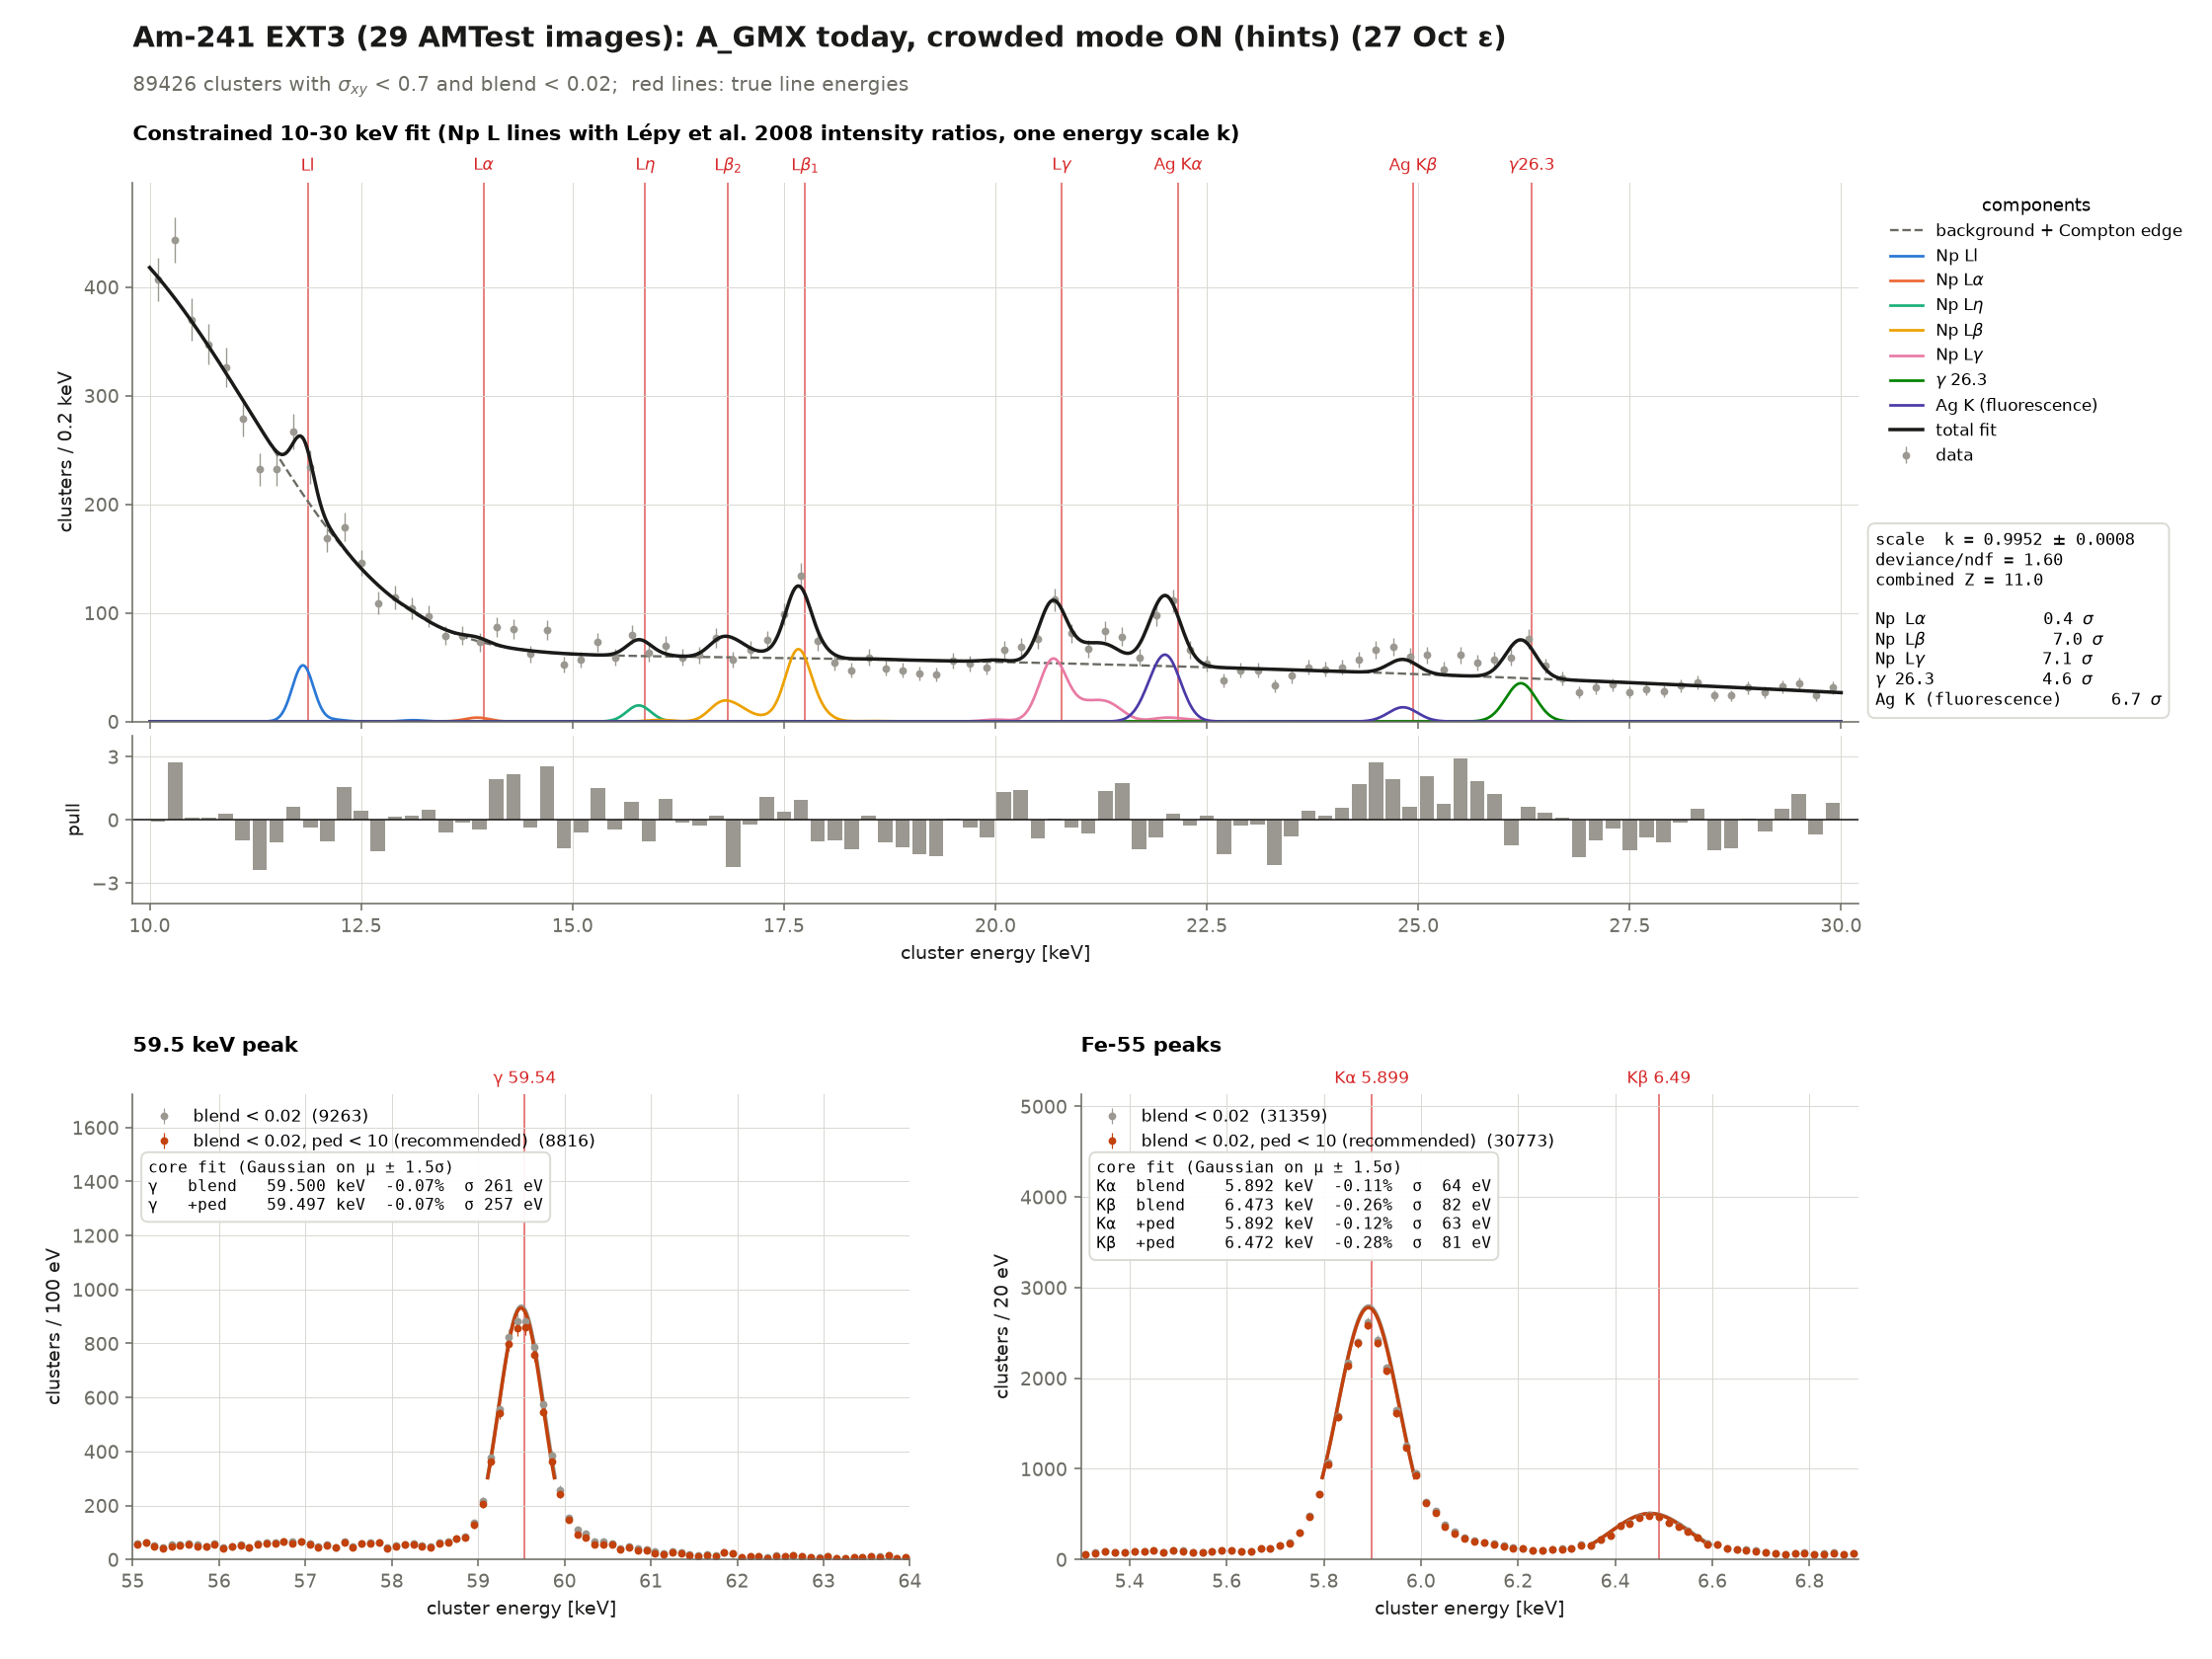
\includegraphics[width=0.49\textwidth]{fit_ext3_on.png}
\caption{EXT3, 29 images, today's code with crowded mode off (left: $k=0.9964\pm0.0010$, deviance/ndf 1.66, $Z=11.3$) and on
(right: $k=0.9952\pm0.0008$, 1.60, $Z=11.0$). The 59.5-keV and Fe-55 peaks move by 3--33\,eV.}
\end{figure}

\subsection{Energy of the straight tracks}
\begin{figure}[H]\centering
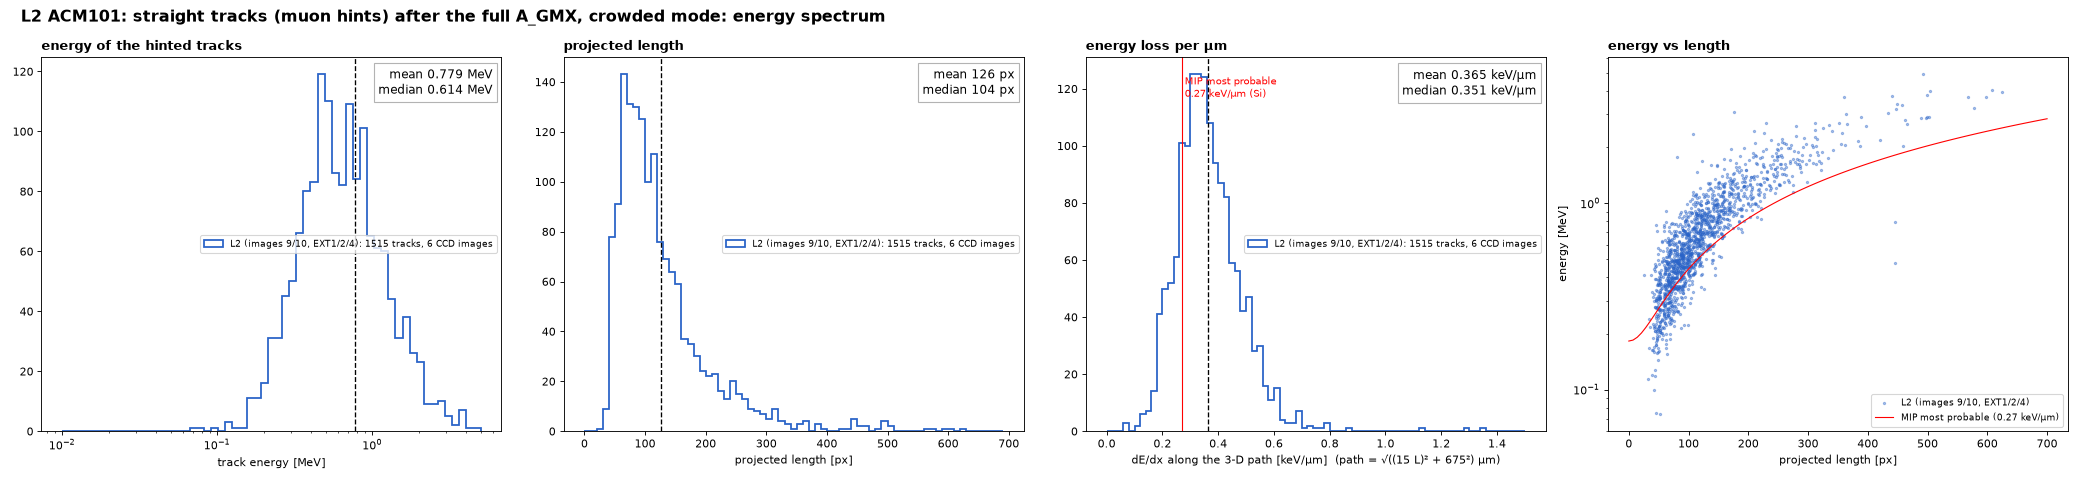
\includegraphics[width=\textwidth]{muon_spectrum.png}
\caption{Clusters defined by the hints: energy, projected length, energy loss along the 3-D path
$\sqrt{(15L)^2+675^2}$\,\textmu m and energy vs length, L2 ACM101. Over 1515 tracks the mean energy is 0.78\,MeV (median 0.61\,MeV) and the most
probable energy loss 0.34\,keV/\textmu m, $\sim$25\,\% above the 0.27\,keV/\textmu m of a minimum-ionising particle: the
clusters also carry their share of the tracks they cross, and some are straight stretches of electron tracks.}
\end{figure}

%======================================================================================================
\section{Open items}\label{sec:open}
\begin{itemize}
\item \textbf{Am-241 EXT3:} 59.5\,keV loses 2.8\,\% of its events with crowded mode (not traced to one piece).
\item \textbf{Fit routine:} \code{amfit.Model.fit} can end in a wide-line minimum; it should also start from narrow widths.
\item \textbf{Electron tracks:} straight 50--90\,px stretches of curly electron tracks are taken as straight tracks.
\item \textbf{Muon energy:} the hinted clusters' energy loss is 25\,\% above the MIP value on L2; how much of it is charge of
crossing tracks has not been measured.
\item \textbf{Validation:} the injected muons are simulated (Moyal fluctuations, linear diffusion); EXT4 was checked on 10 of 29
images.
\end{itemize}

%======================================================================================================
\section{How to run}
\begin{lstlisting}
run_WADERs images.txt --gain-correction --clusterer agmx --agmx-crowded auto   # crowded mode where the core fill >= 0.10
run_AGMX WADERs_analysis_<run> --agmx-crowded on                                # force it on a finished run
AGMX_CROWDED=auto python my_script.py                                           # in python: environment default
\end{lstlisting}
\begin{lstlisting}[language=Python]
import adaptive as AD
clusters, info = AD.adaptive_cluster(Q, valid, engine="gmx", crowded="auto", return_info=True)
info["core_fill"], info["crowded_mode"], info["n_hints"], info["n_streaks"], info["n_linked"], info["bg_override"]
\end{lstlisting}
Each output file records the setting and what ran in \code{agmx\_config} (key \code{crowded\_mode}). Code:
\code{clustering\_tests/crowded.py} (the five pieces), \code{adaptive.py} (the switch), \code{gmx.py}
(\code{general\_cluster(split\_crossings=, hints=)}); tests: \code{tests/test\_agmx\_crowded.py}; the study that led here:
\code{wip/agmx\_crowded/}.
\end{document}
